\documentclass[paper=letter,fontsize=11pt]{scrartcl} % KOMA-article class
							
\usepackage[english]{babel}
\usepackage[utf8x]{inputenc}
\usepackage[protrusion=true,expansion=true]{microtype}
\usepackage{amsmath,amsfonts,amsthm}     % Math packages
\usepackage{graphicx}                    % Enable pdflatex
\usepackage[svgnames]{xcolor}            % Colors by their 'svgnames'
\usepackage{geometry}
	%\textheight=700px                    % Saving trees ;-)
%\usepackage{url}
\usepackage[colorlinks=true, linkcolor=blue, urlcolor=blue]{hyperref}
\usepackage{float}
\usepackage{etaremune}
\usepackage{wrapfig}

\usepackage{attachfile}

% packages I have added
\usepackage{marvosym}
\usepackage[square, numbers]{natbib}

\frenchspacing              % Better looking spacings after periods
\pagestyle{empty}           % No pagenumbers/headers/footers

%\addtolength{\voffset}{-40pt}
%\addtolength{\textheight}{20pt}

\setlength\topmargin{0pt}
\addtolength\topmargin{-\headheight}
\addtolength\topmargin{-\headsep}
\setlength\oddsidemargin{0pt}
\setlength\textwidth{\paperwidth}
\addtolength\textwidth{-2in}
\setlength\textheight{\paperheight}
%\addtolength\textheight{-3in}
\addtolength\textheight{-2in}
\usepackage{layout}

%%% Custom sectioning}{sectsty package)
%%% ------------------------------------------------------------
\usepackage{sectsty}

\sectionfont{%			            % Change font of \section command
	\usefont{OT1}{phv}{b}{n}%		% bch-b-n: CharterBT-Bold font
	\sectionrule{0pt}{0pt}{-5pt}{3pt}}

%%% Macros
%%% ------------------------------------------------------------
\newlength{\spacebox}
\settowidth{\spacebox}{8888888888}			% Box to align text
\newcommand{\sepspace}{\vspace*{1em}}		% Vertical space macro

\newcommand{\MyName}[1]{ % Name
		\Huge \usefont{OT1}{phv}{b}{n} \hfill #1
		\par \normalsize \normalfont}
		
\newcommand{\MySlogan}[1]{ % Slogan}{optional)
		\large \usefont{OT1}{phv}{m}{n}\hfill \textit{#1}
		\par \normalsize \normalfont}

\newcommand{\NewPart}[2]{\section*{\uppercase{#1} #2}}

\newcommand{\PersonalEntry}[2]{
		\noindent\hangindent=2em\hangafter=0 % Indentation
		\parbox{\spacebox}{        % Box to align text
		\textit{#1}}		       % Entry name}{birth, address, etc.)
		\hspace{1.5em} #2 \par}    % Entry value

\newcommand{\SkillsEntry}[2]{      % Same as \PersonalEntry
		\noindent\hangindent=2em\hangafter=0 % Indentation
		\parbox{\spacebox}{        % Box to align text
		\textit{#1}}			   % Entry name}{birth, address, etc.)
		\hspace{1.5em} #2 \par}    % Entry value	
		
\newcommand{\EducationEntry}[4]{
		\noindent \textbf{#1} \hfill      % Study
		\colorbox{White}{%
			\parbox{10em}{%
			\hfill\color{Black}#2}} \par  % Duration
		\noindent \textit{#3} \par        % School
		\noindent\hangindent=2em\hangafter=0 \small #4 % Description
		\normalsize \par}

\newcommand{\WorkEntry}[4]{				  % Same as \EducationEntry
		\noindent \textbf{#1} \hfill      % Jobname
		\colorbox{White}{\color{White}#2} \par  % Duration
		\noindent \textit{#3} \par              % Company
		\noindent\hangindent=2em\hangafter=0 \small #4 % Description
		\normalsize \par}

\newcommand{\PaperEntry}[7]{
		\noindent #1, ``\href{#7}{#2}", \textit{#3} \textbf{#4}, #5 (#6).}

\newcommand{\ArxivEntry}[3]{
		\noindent #1, ``\href{http://arxiv.org/abs/#3}{#2}", \textit{{cond-mat/}#3}.}
        
\newcommand{\BookEntry}[4]{
		\noindent #1, ``\href{#3}{#4}", \textit{#3}.}
        
\newcommand{\FundingEntry}[6]{
        % agency, title portuguese, title english, id, amount, period
        \noindent #1, Title (portuguese): ``#2", Title (english): ``#3", ID: #4, R\$ #5, #6.}

\newcommand{\TalkEntry}[4]{
		\noindent #1, #2, #3 #4}

\newcommand{\ThesisEntry}[6]{
        % type (MSc or PhD), title portuguese, title english, student, institution, year conclusion
		\noindent [#1] Title (portuguese): ``#2", Title (english): ``#3", Student: #4, \textit{#5} (#6).}

\newcommand{\CourseEntry}[5]{
        % level (Graduate or Undergraduate), title, program name, institution, period
		\noindent #1 course: ``#2", #3, \textit{#4}, #5}

%%% Begin Document
%%% ------------------------------------------------------------
\begin{document}

%\layout

\MyName{\begin{flushleft} Vanderlei C. Oliveira Jr. \end{flushleft}}
\MySlogan{\vspace{-0.3in}\begin{flushleft}
{\Large Associate Professor of Geophysics}\\
\vspace{0.1in}
{\Large \Mundus}
\href{http://www.on.br/index.php/pt-br/}{Observat\'{o}rio Nacional},
\href{https://goo.gl/maps/jAEuzxWwPmt}{Rio de Janeiro, RJ, Brazil}\\
{\Large \Letter} \href{mailto:vanderlei@on.br}{vanderlei@on.br}\\
{\Large \Letter} \href{mailto:vandscoelho@gmail.com}{vandscoelho@gmail.com}\\
{\Large \Info} \href{http://www.pinga-lab.org/people/oliveira-jr.html}{pinga-lab.org/people/oliveira-jr}\\
{\Large \Info} \href{http://orcid.org/0000-0002-6338-4086}{orcid.org/0000-0002-6338-4086}
\end{flushleft}}

% you can upload a photo and include it here...
\begin{wrapfigure}{r}{0.3\textwidth}
	%\vspace*{-20em}
	\vspace{-2.9in}
		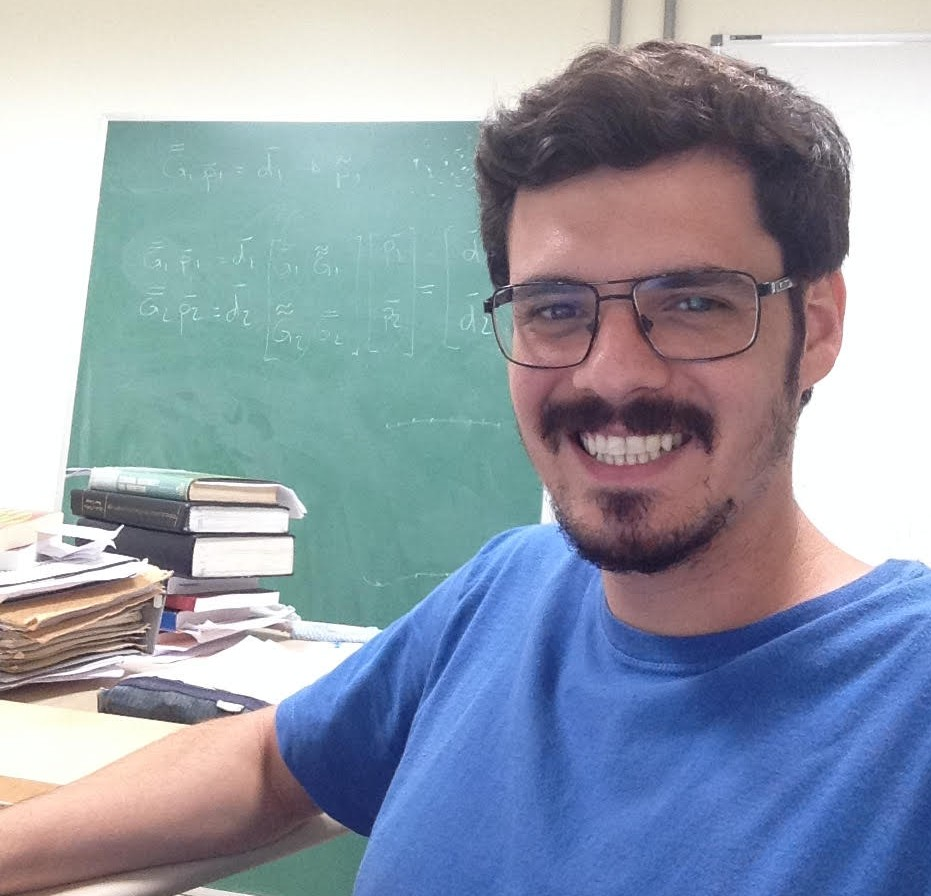
\includegraphics[width=0.3\textwidth]{pictures/vanderlei}
\end{wrapfigure}


\sepspace

\NewPart{Overview}{}
Associate Professor at the geophysics department of Observat\'{o}rio Nacional, Brazil.
Specialist in numerical methods for processing and interpreting potential 
fields (gravity and magnetic).

%%% Personal details
%%% ------------------------------------------------------------
% \NewPart{}{}

% \PersonalEntry{Address}{\href{http://maps.google.com/maps/ms?ie=UTF&msa=0&msid=205373386241137011999.000494c753d05031c4fe4}{Physical Sciences Complex}, University of Maryland, College Park}
% \PersonalEntry{Phone}{(301) 337-7461}
% \PersonalEntry{Mail}{\href{mailto:appelbaum@physics.umd.edu}{appelbaum@physics.umd.edu}}
% \PersonalEntry{WWW}{\href{http://appelbaumlab.umd.edu/CV.html}{http://appelbaum.physics.umd.edu}}


%%% Work experience
%%% ------------------------------------------------------------
\NewPart{Appointments}{}

%\noindent \textbf{Professor of Geophysics} \hfill      % Study
%		\colorbox{White}{%
%			\parbox{6em}{%
%			\hfill\color{Black}2013--}} \par

%\EducationEntry{\textattachfile[color=1 0 1]{research.pdf}{Associate Professor of Physics}}{2009-2016}
%{University of Maryland, College Park}{\begin{itemize}

\EducationEntry{Associate Professor of Geophysics}{2017--}
{Observat\'{o}rio Nacional, Rio de Janeiro, Brazil}

\EducationEntry{Assistant Professor of Geophysics}{2013--2016}
{Observat\'{o}rio Nacional, Rio de Janeiro, Brazil}

\sepspace

\NewPart{Research interests}{}

{\begin{itemize}

\item{\textbf{Equivalent layer technique:} computationally efficient methods for processing and interpreting large potential field data sets.}

\item{\textbf{Inversion of gravity and/or magnetic data:} methods to invert gravity and/or magnetic data for the purpose of estimating the position and shape of geological bodies.}

\item{\textbf{Magnetization of geological bodies:} methods for estimating the magnetization direction of geological bodies by using land and airborne magnetic data.}

\item{\textbf{Magnetization of rock samples:} methods for estimating the magnetization distribution within rock samples by using scanning magnetic microscopy data.}

\item{\textbf{Magnetic modelling of geological bodies:} methods for computing the demagnetizing field within geological bodies having high susceptibility.}

\item{\textbf{Regional characterization of gravity field:} computationally efficient methods for representing the regional gravity field by combining different data sets.}

\item{\textbf{Regional characterization of the crustal magnetic field:} computationally efficient methods for representing the crustal field by combining different data sets.}

\end{itemize}}

\sepspace

%%% Education
%%% ------------------------------------------------------------
\NewPart{Education}{}

\EducationEntry{\Large PhD Geophysics}{\begin{flushright} Dec/2010 -- Jan/2013 \end{flushright} \vspace{-0.2in}}{\href{http://www.on.br/index.php/pt-br/}{Observat\'{o}rio Nacional}, Brazil}

\sepspace \noindent
\textbf{Title (portuguese):} \href{http://www.pinga-lab.org/thesis/oliveira-jr-phd.html}{``Processamento e invers\~{a}o de dados de campos potenciais: Novas abordagens"} \\
\textbf{Title (english):} ``Processing and inversion of potential field data: New approaches" \\
\textbf{Advisor:} Dr. Valeria C. F. Barbosa \\
\textbf{Descritpion:} This work presents two new methodologies for processing and interpreting potential field data. The first one is the Polynomial Equivalent Layer, which is a cost-effective method for processing large potential-field data sets via the equivalent-layer technique. The second is a non-linear method for inverting gravity-gradient data to estimate the shape of isolated 3-D geological bodies.

\sepspace

\EducationEntry{\Large MSc Geophysics}{\begin{flushright} Mar/2009 -- Nov/2010 \end{flushright} \vspace{-0.2in}}{\href{http://www.on.br/index.php/pt-br/}{Observat\'{o}rio Nacional}, Brazil}

\sepspace \noindent
\textbf{Title (portuguese):} \href{http://www.pinga-lab.org/thesis/oliveira-jr-msc.html}{``Invers\~{a}o gravim\'{e}trica radial por camadas para a reconstru\c{c}\~{a}o de corpos geol\'{o}gicos 3D"} \\
\textbf{Title (english):} ``Radial gravity inversion by layers for retrieving 3D geological bodies" \\
\textbf{Advisor:} Dr. Valeria C. F. Barbosa \\
\textbf{Descritpion:} This work presents a gravity-inversion method for estimating the geometry of a 3D source. The subsurface region containing the geologic source is discretized into an ensemble of vertically juxtaposed prisms. By estimating the coordinates of the horizontal section of each prism, the method retrieves a set of polygonal horizontal sections representing depth slices of the 3D gravity source.

\sepspace

\EducationEntry{\Large BSc Geophysics}{\begin{flushright} Mar/2004 -- Dec/2008 \end{flushright} \vspace{-0.2in}}{\href{http://www.iag.usp.br/international/}{University of S\~{a}o Paulo}, Brazil}

\sepspace \noindent
\textbf{Title (portuguese):} ``Modelagem gravim\'{e}trica 3D da borda norte da Bacia do Paran\'{a}" \\
\textbf{Title (english):} ``3D gravity modelling of the northern border of the Paran\'{a} basin" \\
\textbf{Advisor:} Dr. Yara R. Marangoni \\
\textbf{Descritpion:} This work presents a geological model of the northern border of the Paran\'{a} basin obtained from gravity data.

\sepspace

%%% Papers
%%% ------------------------------------------------------------

%\NewPart{Peer-Reviewed Journal Papers}{( \href{http://orcid.org/0000-0002-6338-4086}{ORCID} )}
\renewcommand{\refname}{PEER-REVIEWED JOURNAL PAPERS (\href{http://orcid.org/0000-0002-6338-4086}{ORCID})}

% list of papers
% list of papers

\nocite{*}
\bibliographystyle{cv}
%\bibliography{papers}
\begin{thebibliography}{10}

\bibitem{araujo_hallsensor_2019}
J.~Araujo, A.~Reis, V.~C. Oliveira{ }Jr, A.~Santos, C.~Luz-Lima, E.~Yokoyama,
  L.~Mendoza, J.~Pereira, A.~Bruno. Characterizing Complex Mineral Structures
  in Thin Sections of Geological Samples with a Scanning Hall Effect
  Microscope. \emph{Sensors} \textbf{2019}, \emph{19}, 1636.

\bibitem{takahashi_ellipsoids_2017}
D.~Takahashi, V.~C. Oliveira~Jr. Ellipsoids (v1.0): 3-{D} magnetic modelling of
  ellipsoidal bodies. \emph{Geoscientific Model Development} \textbf{2017},
  \emph{10}, 3591--3608.

\bibitem{siqueira_fast_2017}
F.~C.~L. Siqueira, V.~C. Oliveira~Jr., V.~C.~F. Barbosa. Fast iterative
  equivalent-layer technique for gravity data processing: {A} method grounded
  on excess mass constraint. \emph{GEOPHYSICS} \textbf{2017}, \emph{82},
  G57--G69.

\bibitem{reis_estimating_2016}
A.~L.~A. Reis, V.~C. Oliveira~Jr., E.~Yokoyama, A.~C. Bruno, J.~M.~B. Pereira.
  Estimating the magnetization distribution within rectangular rock samples.
  \emph{Geochemistry, Geophysics, Geosystems} \textbf{2016}, \emph{17},
  3350--3374.

\bibitem{oliveira_jr_estimation_2015}
V.~Oliveira~Jr, D.~Sales, V.~Barbosa, L.~Uieda. Estimation of the total
  magnetization direction of approximately spherical bodies. \emph{Nonlinear
  Processes in Geophysics} \textbf{2015}, \emph{22}, 215--232.

\bibitem{uieda_geophysical_2014}
L.~Uieda, V.~C. Oliveira~Jr., V.~C.~F. Barbosa. Geophysical tutorial: {Euler}
  deconvolution of potential-field data. \emph{The Leading Edge} \textbf{2014},
  \emph{33}, 448--450.

\bibitem{melo_estimating_2013}
F.~F. Melo, V.~C.~F. Barbosa, L.~Uieda, V.~C. Oliveira~Jr., J.~B.~C. Silva.
  Estimating the nature and the horizontal and vertical positions of 3D
  magnetic sources using {Euler} deconvolution. \emph{GEOPHYSICS}
  \textbf{2013}, \emph{78}, J87--J98.

\bibitem{oliveira_3-d_2013}
V.~C. Oliveira~Jr., V.~C. Barbosa. 3-{D} radial gravity gradient inversion.
  \emph{Geophysical Journal International} \textbf{2013}, \emph{195}, 883--902.

\bibitem{oliveira_jr._polynomial_2013}
V.~C. Oliveira~Jr., V.~C.~F. Barbosa, L.~Uieda. Polynomial equivalent layer.
  \emph{GEOPHYSICS} \textbf{2013}, \emph{78}, G1--G13.

\bibitem{oliveira_jr_source_2011}
V.~C. Oliveira~Jr., V.~C.~F. Barbosa, J.~B.~C. Silva. Source geometry
  estimation using the mass excess criterion to constrain 3-{D} radial
  inversion of gravity data. \emph{Geophysical Journal International}
  \textbf{2011}, \emph{187}, 754--772.

\end{thebibliography}



%%% International Conferences
%%% ------------------------------------------------------------

\renewcommand{\refname}{LAST PARTICIPATIONS AT INTERNATIONAL CONFERENCES}

% list of conferences
% list of conferences

\nocite{*}
\bibliographystyle{cv}
%\bibliography{conferences}
\begin{thebibliography}{10}
\providecommand{\natexlab}[1]{#1}
\expandafter\ifx\csname urlstyle\endcsname\relax
  \providecommand{\doi}[1]{doi:\discretionary{}{}{}#1}\else
  \providecommand{\doi}{doi:\discretionary{}{}{}\begingroup
  \urlstyle{rm}\Url}\fi

\bibitem[{Reis and Oliveira~Jr.(2017)}]{latinmag_2017}
Reis, A. L.~A. and Oliveira~Jr., V.~C.
\newblock Sed for optimal acquisition design and sensor-to-sample distance
  applied to scanning magnetic microscopy.
\newblock In \emph{Fifth bi-anual meeting of the LATINMAG}. LATINMAG,
  Quer\'{e}taro, M\'{e}xico, 2017.
\newblock [abstract co-author].

\bibitem[{Hallam and Oliveira~Jr.(2016)}]{agu_fallmeeting_2016b}
Hallam, K. A.~T. and Oliveira~Jr., V.~C.
\newblock Applications of differential operators in geodetic coordinates.
\newblock In \emph{2016 AGU Fall Meeting}. AGU, San Francisco, USA, 2016.
\newblock [attendee, abstract co-author].

\bibitem[{Reis and Oliveira~Jr.(2016)}]{agu_fallmeeting_2016a}
Reis, A. L.~A. and Oliveira~Jr., V.~C.
\newblock Impact of the sensor area, acquisition design and position noise on
  the estimation of the magnetization distribution within a rectangular rock
  sample.
\newblock In \emph{2016 AGU Fall Meeting}. AGU, San Francisco, USA, 2016.
\newblock [attendee, abstract co-author].

\bibitem[{Oliveira~Jr. et~al.(2015)Oliveira~Jr., Sales, Barbosa, and
  Uieda}]{iugg_2015a}
Oliveira~Jr., V.~C., Sales, D.~P., Barbosa, V. C.~F., and Uieda, L.
\newblock Estimating the total magnetization direction of approximately
  spherical bodies.
\newblock In \emph{26th IUGG General Assembly - IAGA - A41 Lithospheric Field
  Modeling, the WDMAM and Tectonic Implications (Div. V) - A41p-280}. IUGG,
  Prague, Czech Republic, 2015.
\newblock [attendee, abstract co-author, poster presenter].

\bibitem[{Reis et~al.(2015)Reis, Oliveira~Jr., Yokoyama, Bruno, and
  Pereira}]{iugg_2015b}
Reis, A. L.~A., Oliveira~Jr., V.~C., Yokoyama, E., Bruno, A.~C., and Pereira,
  J. M.~B.
\newblock Estimating the magnetization distribution within rectangular rock
  samples.
\newblock In \emph{26th IUGG General Assembly - IAGA - A06d-A06d A06/A07
  Applied Rock Magnetism (Div. I) / Theoretical and Experimental Rock Magnetism
  (Div. I) - IUGG-1853}. IUGG, Prague, Czech Republic, 2015.
\newblock [attendee, abstract co-author, oral presenter].

\bibitem[{Oliveira~Jr. and Barbosa(2014)}]{eage_2014}
Oliveira~Jr., V.~C. and Barbosa, V. C.~F.
\newblock 3-d radial gravity gradient inversion applied to the interpretation
  of the vinton salt dome, usa.
\newblock In \emph{76th EAGE Conference and Exhibition 2014}. EAGE, Amsterdam,
  Netherlands, 2014.
\newblock [attendee, expanded abstract author, oral presenter].

\bibitem[{Uieda et~al.(2013)Uieda, Oliveira~Jr., and Barbosa}]{scipy_2013}
Uieda, L., Oliveira~Jr., V.~C., and Barbosa, V. C.~F.
\newblock Modeling the earth with fatiando a terra.
\newblock In \emph{12th Scientific Computing with Python Conference}. SciPy,
  Austin, USA, 2013.
\newblock [expanded abstract co-author].

\bibitem[{Oliveira~Jr. and Barbosa(2012)}]{seg_2012}
Oliveira~Jr., V.~C. and Barbosa, V. C.~F.
\newblock Polynomial equivalent layer.
\newblock In \emph{SEG Las Vegas 2012 Annual Meeting}. SEG, Las Vegas, USA,
  2012.
\newblock [expanded abstract author].

\bibitem[{Oliveira~Jr. and Barbosa(2011{\natexlab{a}})}]{eage_2011}
Oliveira~Jr., V.~C. and Barbosa, V. C.~F.
\newblock 3d radial inversion of gravity data for estimating the source's
  geometry.
\newblock In \emph{73rd EAGE Conference and Exhibition incorporating SPE
  EUROPEC 2011}. EAGE, Vienna, Austria, 2011{\natexlab{a}}.
\newblock [attendee, expanded abstract author, oral presentation].

\bibitem[{Oliveira~Jr. and Barbosa(2011{\natexlab{b}})}]{seg_2011}
Oliveira~Jr., V.~C. and Barbosa, V. C.~F.
\newblock Radial gravity inversion constrained by total anomalous mass excess
  for retrieving 3d bodies.
\newblock In \emph{SEG San Antonio 2011 Annual Meeting}. SEG, San Antonio, USA,
  2011{\natexlab{b}}.
\newblock [expanded abstract author].

\end{thebibliography}


\NewPart{Theses Supervised}{}

\begin{enumerate}

\item\ThesisEntry{MSc}{\href{http://www.pinga-lab.org/thesis/takahashi-msc.html}{Modelagem magn\'{e}tica 3D de corpos elipsoidais}}{3D Magnetic modeling of elipsoidal bodies}{Diego Takahashi}{Observat\'{o}rio Nacional, Brazil}{2017}

\item\ThesisEntry{MSc}{\href{http://www.pinga-lab.org/thesis/andre-msc.html}{Invers\~{a}o magn\'{e}tica 3D para estimar a distribui\c{c}\~{a}o de magnetiza\c{c}\~{a}o de uma amostra de rocha}}{3D Magnetic inversion to estimate the magnetization distribution of a rectangular rock sample}{Andr\'{e} L. A. Reis}{Observat\'{o}rio Nacional, Brazil}{2016}

\item\ThesisEntry{MSc}{\href{http://www.pinga-lab.org/thesis/daiana-msc.html}{Estimativa do vetor de magnetiza\c{c}\~{a}o total de corpos aproximadamente esf\'{e}ricos}}{Estimating the total magnetization vector of approximately spherical bodies}{Daiana P. Sales}{Observat\'{o}rio Nacional, Brazil}{2014}

\end{enumerate}

\sepspace

\NewPart{Theses Co-supervised}{}

\begin{enumerate}

\item\ThesisEntry{MSc}{Investiga\c{c}\~{a}o geof\'{i}sica do Alto do Cear\'{a} na margem equatorial brasileira -- Uma crosta continental ou uma crosta oce\^{a}nica?}{Geophysical investigation of the Cear\'{a} Rise in the brazilian equatorial margin -- A continental crust or oceanic crust?}{Victor C. Pereira}{Observat\'{o}rio Nacional, Brazil}{2017}

\item\ThesisEntry{PhD}{\href{http://www.pinga-lab.org/thesis/siqueira-phd.html}{Otimiza\c{c}\~{a}o computacional do m\'{e}todo da camada equivalente}}{Computational optimization of the equivalent layer method}{Fillipe C. L. Siqueira}{Observat\'{o}rio Nacional, Brazil}{2016}

\end{enumerate}

\sepspace

\NewPart{Teaching}{}

\begin{itemize}

\item\CourseEntry{Graduate}{Potential-field methods}{Graduation Program in Geophysics}{Observat\'{o}rio Nacional, Brazil}{2014 -- present}

\item\CourseEntry{Graduate}{Computational methods applied to Geophysics}{Graduation Program in Geophysics}{Observat\'{o}rio Nacional, Brazil}{2014 -- present}

\end{itemize}

\sepspace

\NewPart{Participation in departmental committees}{}

\begin{itemize}

\item Head of the academic staff of the Graduate Program in Geophysics of the 
Observat\'{o}rio Nacional, 2017 -- present

\item Member of the academic staff of the Graduate Program in Geophysics of the 
Observat\'{o}rio Nacional, 2014 -- present

\end{itemize}

\sepspace

\NewPart{Funding}{}

\begin{itemize}

\item\FundingEntry{\href{http://cnpq.br/pagina-inicial}{Conselho Nacional de Desenvolvimento Cient\'{i}fico e Tecnol\'{o}gico (CNPq)}}{Estimativa da dire\c{c}\~{a}o da magnetiza\c{c}\~{a}o total de corpos 3D aproximadamente esf\'{e}ricos}{Estimation of the total magnetization direction of approximately 3D spherical bodies}{445752/2014-9}{20~000.00}{Nov/2014 -- Nov/2017}

\item\FundingEntry{\href{http://www.faperj.br/}{Funda\c{c}\~{a}o Carlos Chagas Filho de Amparo \`{a} Pesquisa do Estado do Rio de Janeiro (FAPERJ)}}{Infraestrutura computacional para a estima\c{c}\~{a}o da magnetiza\c{c}\~{a}o de corpos 3D aproximadamente dipolares}{Computational infrastructure for estimating the magnetization direction of approximately dipolar bodies}{E-26/111.152/2014}{10~000.00}{Jun/2014 -- Mar/2016}

\end{itemize}

%\NewPart{Invited Talks at International Conferences}{}
%\begin{etaremune}
%\item\TalkEntry{Nano-Spin Conversion Workshop}{RIKEN Tokyo}{10/16}{(declined)} 
%\item\TalkEntry{APS March meeting}{Baltimore}{3/16}{} 
%\item\TalkEntry{APS Mid Atlantic Section Meeting}{Morgantown, WV}{10/15}{} 
%\item\TalkEntry{MMM-2014}{Honolulu}{11/14}{ (by postdoc Pengke Li)} 
%\end{etaremune}


%\NewPart{Synergistic Activities}{}
%\begin{itemize}
%\item Proposal reviewer: NSF (ECCS panel 9/08, 1/10, 5/11, 11/12, 2/16), Research Corporation, DOE, EPSCoR, Defense Threat Reduction Agency, Science Foundation Ireland, Icelandic Centre for Research, Israel Science Foundation, Austrian Science Fund
%\item Referee: Nature Physics, Nature Nanotech, Nature Materials, Physical Review Letters, Physical Review B, Applied Physics Letters, Europhysics Letters, Journal of Applied Physics, J. Magn. Magn. Mat., Semiconductor Sci. and Tech., etc.
%\item Proposed and chaired 2015 APS March meeting invited symposium session, \href{http://meeting.aps.org/Meeting/MAR15/Session/Y20}{Spin Accumulation: Experiment and Theory Behind the Controversy}.
%\item Tutorial Instructor and session chair: \href{http://appelbaum.physics.umd.edu/docs/ppt/Appelbaum_102414.pdf}{``Spintronics"}, APS March meeting (2014), Spin Transport Physics short course, DRC (2010).
%\item Program Committee: 12th Joint MMM/Intermag (2013), PASPS-7 (Eindhoven August 5-8 2012), 2010 and 2011 Electronic Materials Conference, Device Research Conference (2009, 2010 and 2011), Focus Session on Spin Dependent Phenomena in Semiconductors, APS March meeting (2009), Chinese-American Kavli Frontiers in Science Symposium, US National Academy of Sciences (2008)
%\item Five lectures viewed by over 3000 students worldwide on coursera.org MOOC \href{https://www.coursera.org/course/eqp}{``Exploring Quantum Physics"}
%\item U.S. Patent 7244997, ``\href{http://www.google.com/patents/US7244997}{Magneto-Luminescent Transducer}"
%\item Life Member 61024031, American Physical Society
%\end{itemize}

%\NewPart{Awards}{}
%\begin{itemize}
%\item 2016 \href{https://www.aps.org/programs/honors/fellowships/archive-all.cfm?initial=&year=2016&unit_id=DCMP&institution=University+of+Maryland%2C+College+Park}{Fellow, American Physical Society}: “\textit{For advancing the study of spin-polarized electron transport in semiconductors, especially the fundamental processes revealed by coherent and time-resolved spin transport over macroscopic distances in silicon and germanium.}”
%\item 2011 \href{http://www.mdsci.org/programs/outstanding-young-scientist-outstanding-young-engineer/past-oys-recipients/}{A.M. Haig prize / Outstanding Young Scientist}, MD Academy of Sciences
%%\item 2010 \textattachfile[color=1 0 1]{IUPAP.jpg}{``Highly Commended"}:  IUPAP Young Scientist Prize in Semiconductor Physics 
%\item 2009 NSF CAREER award
%\item 2008 Outstanding Junior Faculty Member for the College of Engineering (Delaware)
%\item 2007 Cambridge NanoTech Research Award 
%\item 1998 G. Howard Carragan Award (RPI) ``For outstanding scholarship"
%\item 1998 Hertz Foundation - Grant recipient
%\item 1996 Rensselaer Founder's Award
%\end{itemize}

\end{document}
